\documentclass{article}

\usepackage[english]{babel}
\usepackage[utf8]{inputenc}
\usepackage{amsthm}
\usepackage{amsmath}
\usepackage{amssymb}
\usepackage{geometry}
\usepackage{graphicx}
\usepackage{csquotes}


\graphicspath{{./}}

\newtheorem*{theorem}{Theorem}
\newtheorem*{definition}{Definition}
\newtheorem*{lemma}{Lemma}
\newtheorem*{proposition}{Proposition}
\newtheorem*{conjecture}{Conjecture}
\newtheorem*{observation}{Observation}
\newtheorem*{corollary}{Corollary}

\newcommand{\R}{\mathbb{R}}

\title{Polyhedral combinatorics -- Lecture 11}
\author{Filip Kastl}
\date{\today}


\begin{document}

\maketitle

\noindent
\emph{version 1 -- \today}

\section{Non-negative rank (propositions from the tutorial)}

\begin{definition}[Non-negative rank]
	The \emph{non-negative rank} $rk_+(M)$ for $M_{m \times n} \ge 0$ is
	defined as
	$$
	rk_+(M) = \min \{ r ~|~ \exists T_{m \times r} \ge 0, U_{r \times n}
	\ge 0 ~s.t.~ M = TU \}
	$$
\end{definition}

\begin{proposition}
	$rk_+(M)$ is equal to the minimum number of rank-1 non-negative
	matrices that sum to $M$.
\end{proposition}

\begin{observation}
	~
	\begin{itemize}
		\item The non-negative rank of a matrix is at least as large as
			its rank
		\item The non-negative rank of a matrix is at most as large as
			the minimum number of rows and columns of the matrix.
		\item The non-negative rank of a matrix is equal to the
			non-negative rank of its transpose.
	\end{itemize}
\end{observation}

\begin{proposition}
	The non-negative rank of the product of two matrices $A$ and $B$ is at
	most as large as the minimum of the non-negative rank of $A$ and the
	non-negative rank of $B$.
\end{proposition}

\begin{proposition}
	The non-negative rank of the sum of two matrices $A$ and $B$ is at most
	as large as the sum of the non-negative rank of $A$ and the
	non-negative rank of $B$.
\end{proposition}


\section{Yannakakis theorem}

Say we have a problem of size $n$. We search for a polyhedron representing the
problem and its description using linear equalities and inequalities. We might
end up with exponentially many inequalities \footnote{I'd like to stress that
we only count the number of inequalities. The equalities don't bother us. I was
confused by that. Not sure why inequalities are so much of a bigger deal. I
guess that you can first solve the equality part of the polyhedron by
polynomial linear algebra methods and then deal with the inequalities?}. We
might search for other descriptions of the polyhedron in $\R^d$ with
polynomially many inequalities. If that doesn't work out, another approach is
to search for polyhedrons of higher dimension whose projection to $\R^d$ is
equivalent to the original polyhedron.


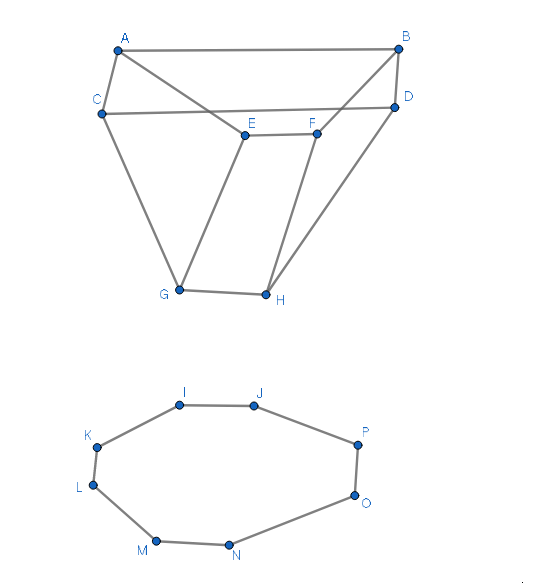
\includegraphics[width=200px]{extended-formulation.png}

\begin{definition}[Extended formulation]
	Let $P \subseteq \R^d, P = \{x | \hdots\}$ and $Q \subseteq \R^{d + r},
	Q = \{(x, y) | \hdots\}$ be polytopes.

	$Q$ is an extended formulation of $P$ if $P = \Pi_x(Q) := \{ x |
	\exists y: (x, y) \in Q\}$
\end{definition}

\begin{definition}[Extension complexity]
	The \emph{extension complexity} $xc(P) =$ min number of inequalities
	describing any extended formulation of $P$.
\end{definition}

\begin{definition}[Slack matrix]
	Let $P = \{x|A_{m \times d}x \le b\} = conv(V_{n \times d})$.

	The non-negative \emph{slack matrix} $S(P)$ is an $m \times n$ matrix
	s.t.
	$$
	S_{ij} = b_i - a_i^Tv_j
	$$
\end{definition}

The following theorem is important because it enables us to go from bounds on
the non-negative rank to bounds on $xc$.

\begin{theorem}[Yannakakis]
	Let $P$ be a polytope. Then $xc(P) = rk_+(S(P))$.
\end{theorem}
\begin{proof}
	~

	\emph{reference: Mihalis Yannakakis: Expressing Combinatorial
	Optimization Problems by Linear Programs, Theorem 3}

	\noindent
	\enquote{$\le$}

	Let's show that for a given slack matrix $S(P)$ of non-negative rank
	$r$ we can construct an extended formulation $Q$ of the polytope $P$.
	Let $P = \{ x | A_{m \times n}x \le b\}$ (WLOG there are no
	equalities). Let $S(P) = T_{m \times r}U_{r \times n}$ be a
	non-negative factorization of the slack matrix $S(P)$. We define the
	extended formulation as follows
	$$
	Q := \{(x,y) | Ax + Ty = b, y \ge 0\}
	$$
	So $Q$ only has $r$ inequalities ($y \ge 0$).

	Now let's show that $Q$ is really an extended formulation of $P$ --
	show that $\Pi_x (Q) = P$.

	\begin{itemize}
		\item \enquote{$\subseteq$}
			Let $x,y \in Q$. By definition of $Q$ it holds that $Ax
			+ Ty = b$. Because $T$ is non-negative it holds that
			$Ty \ge 0$. That means that $Ax \le b$ which by
			definition means that $x \in P$.
		\item \enquote{$\supseteq$}
			Let's show that for each vertex $v_i$ of $P$ exists $y$
			s.t. $(v_i,y) \in Q$. This will suffice since points of
			$P$ are convex combinations of vertices and those
			will then translate to convex combinations of points of
			$Q$.

			Let's use $y := U_{*i}$. For each $i$, $(v_i, U_{*i})$
			is a feasible solution of $Ax + Ty = b, y \ge 0$
			because $TU_{*i} = S_{*i}$, which is exactly the slack
			of vertex $v_i$.
	\end{itemize}

	\noindent
	\enquote{$\ge$}

	Let $P = \{ x | Ax \le b \} = conv(V)$ and let $Q = \{(x,y) | Ex + Fy
	\le g\}$ be its extended formulation with $r$ inequalities. Note that
	$\forall i: a_i^Tx \le b_i$ is a valid inequality for $Q$. For each of
	these inequalities it should be possible to express them as
	non-negative linear combinations of the inequalities of $Q$
	\footnote{This intuitively makes sense to me but I wouldn't be able to
	prove it. In the lecture this was handwaved as a consequence of
	duality.}. Let's denote the coefficients of these linear combinations
	as
	$\lambda_1^i,...,\lambda_r^i, \lambda_k^i \ge 0$.

	$$
	(a_i, 0) = \sum_{k} \lambda_k^i (E_{k*}, F_{k*})
	$$

	$$
	b_i = \sum_k \lambda_k^i g_k
	$$

	Notice that for a vertex $v$ of $P$ there is a point $(v, u)$ of $Q$
	s.t. the inequality $a_ix \le b_i$ has the same slack w.r.t. $v$ and
	$(v, u)$. In the lecture we assumed that $(v, u)$ is a vertex of $Q$.
	Let me give an explanation of why we can assume this. We can observe
	that $(v, u)$ lies on a facet -- $v$ is an extreme point of $P$ w.r.t.
	some direction and optimizing along this direction gives us a facet of
	$Q$. All of the points of the facet will have the form $(v, y)$ for
	some $y$. This facet will contain some vertices of $Q$. Let $(v, u)$ be
	one of these vertices. Let's now continue with the proof.

	Slack of the inequality of $P$ $a_i^Tx \le b_i$ with respect to vertex
	$v_j$ of $P$ is the same as the slack of the inequality $a_i^Tx \le
	b_i$ that we constructed from inequalities of $Q$ w.r.t. a vertex
	$(v_j, u_j)$ of $Q$ and that can be expressed as the slack of $\sum_{k
	= 1}^r \lambda_k^i \cdot (E_ix + F_iy \le g_i)$ w.r.t. $(v_j, u_j)$.
	Since when you combine inequalities you also combine slack, we finaly
	get this: $\sum_{k = 1}^r \lambda_k^i \cdot ($ slack of $E_ix + F_iy
	\le g_i$ w.r.t. $(v_j, u_j))$.

	Now let's define the non-negative matrices that form the rank $r$
	factorization of $S(P)$. One of them will be $\Lambda$ whose rows are
	the coefficient vectors $\lambda^i$. The second will be submatrix $S$
	of the slack matrix of $Q$ consisting of those columns of $Q$
	corresponding to vertices $(v_j, u_j)$. Both matrices are non-negative,
	have the right number of rows and columns and due to what we have shown
	in the previous paragraph, $\Lambda S = S(P)$.
\end{proof}

In particular, this means that all possible slack matrices of $P$ will have the
same non-negative rank.


\section{Communication complexity}

We now sidestep into the theory of communication complexity. We will show that
a specific type of a communication complexity problem can be used to bound the
non-negative rank of matrix. That will in turn be useful for us when we try to
bound the extension complexity of some combinatorial problems.

\textbf{Communication complexity scenario}. Let $M_{m \times n}$ be a
non-negative matrix. There are two parties: Alice and Bob. Alice gets a row
index $i$ and Bob gets a column index $j$. They communicate and then one of
them outputs a number $X_{ij}$. Their task is to match $M_{ij}$.

We count the number of bits exchanged. For a given matrix $M$ the
\emph{communication complexity} of a communication protocol is the maximum
number of bits exchanged over all $i,j$. The \emph{communication complexity} of
the matrix $M$ ($cc(M)$) is the minimum number of bits exchanged over all
possible communication protocols.

We will concern ourselves with a variant of this problem where the
communication protocol can make decisions base on chance, $X_{ij}$ is a random
variable and the goal is $\mathbb{E}[X_{ij}] = M_{ij} ~\forall i,j$. We will
denote the communication complexity of this problem as $cc_+(M)$.

\begin{definition}[Communication protocol (formally)]
	A \emph{communication protocol} is a binary tree with internal nodes
	labeled Alice/Bob. The leaves represent output. The left downwards edge
	represents sending the other party a 0 bit, the right downwards edge
	represents sending the other party a 1 bit.

	For the probabilistic version of the problem each internal node labeled
	Alice has a probability $p(i) \in [0, 1]$ of sending the 0 bit
	dependent on the row index $i$ asociated with it and each internal node
	labeled Bob has a probability $p(j) \in [0, 1]$ of sending the 0 bit
	dependent on the column index $j$ asociated with it.
\end{definition}

\begin{theorem}
	$\log (rk_+(M)) \sim cc_+(M)$
\end{theorem}

We leave this theorem without a proof for now. The proof will be presented in
the next lecture. Instead, we present an example of usage of this theorem.


\section{The spanning tree polytope}

Let $G = (V, E)$ be a graph. We call the polytope $P_{ST}(G) = \{ \chi^{E'} \in
\{0, 1\}^{|E|} | E'$ is a spanning tree of $G \}$ the \emph{spanning tree
polytope} of $G$. Here is a description of the polytope using linear
inequalities:

$$
\left \{
\begin{array}{c|ccc}
	~ & \sum_{e \in E} x_e = n - 1   & ~ \\
	x & x_e \ge 0                     & \forall e \in E \\
	~ & \sum_{e \in E[U]} \le |U| - 1 & \forall U \subseteq V
\end{array}
\right \}
$$

The third system of inequalities basically says that each subset of vertices
should induce a forest in the spanning tree $E'$.

How does the slack matrix of this polytope look like? It has one column for
each possible spanning tree of $G$. The rows of the slack matrix corresponding
to the first two systems of inequalities are trivial. For the first system we
get all zeros. For the second system we get a row for each edge $e$ where
positions represent whether $e$ is contained in the spanning tree corresponding
to the column.

The part of the matrix corresponding to the third set of inequalities is more
interesting. Rows correspond to subsets $U \subseteq V$. Here is a formula for
elements of this part of the matrix:

$$
S(U, T) = \left ( |U| - 1 - \sum_{e \in E[U]} [e \in T] \right ) - 1
$$

This can be interpreted as $( \#$ components in $T[U]) - 1$.

\subsection{Communication protocol}

\emph{reference: \enquote{basics} paper, section 5.2}

\noindent
Let's bound the extension complexity of the spanning tree polytope by
constructing a communication protocol for its slack matrix.

Let $G = (V, E)$ be a graph. $P_{ST}(G)$ is its spanning tree polytope. In
terms of the corresponding communication problem, Alice has a proper nonempty
set $U \subsetneq V$ and Bob a spanning tree $T$. Together, they wish to
compute $S(U, T)$.

Alice sends the name of some (arbitralily chosen) vertex $u$ of $U$. Then Bob
picks an edge $e$ of $T$ uniformly at random and sends to Alice the endpoints
$v$ and $w$ of $e$ as an ordered pair of vertices $(v, w)$, where the order is
chosen in such a way that $w$ is on the unique path from $v$ to $u$ in the
tree. That is, she makes sure that the directed edge $(v, w)$ \enquote{points}
towards the root $u$. Then Alice checks that $v \in U$ and $w \notin U$, in
which case she outputs $n - 1$; otherwise she outputs $0$.

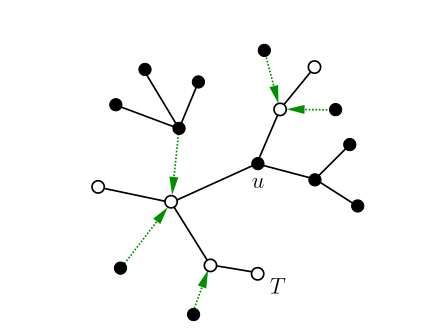
\includegraphics[width=200px]{spanning-tree.png}

The resulting randomized protocol is clearly of complexity $\log |V| + \log |E|
+ O(1)$. Moreover, it computes the slack matrix in expectation because for each
connected component of $T[U]$ distinct from that which contains $u$, there is
exactly one directed edge $(v, w)$ that will lead Alice to output a non-zero
value. Since she outputs $(n - 1)$ in this case, the expected value of the
protocol on pair $(U, T)$ is $(n - 1) \cdot (k - 1)/(n-1) = k - 1$, where $k$
is the number of connected components of $T[U]$. Therefore we obtain the
following result.

\begin{proposition}
	For every graph $G$ with $n$ vertices and $m$ edges, $xc(P_{ST}(G)) \in
	O(mn)$
\end{proposition}

\end{document}
